%\documentclass[SE,toc]{lsstdoc}
\documentclass[SE,lsstdraft,authoryear,toc]{lsstdoc}
\usepackage{hyperref}
% lsstdoc documentation: https://lsst-texmf.lsst.io/lsstdoc.html

% Generated by Makefile
\input{meta}

% Package imports go here.

% Local commands go here.

% If you want glossaries, uncomment:
% \input{aglossary.tex}
% \makeglossaries

\title{SIT-Com Management Plan}
% \setDocSubtitle{Optional subtitle}

\author{%
Charles (Chuck) Claver, Patrick Ingraham
}

\setDocRef{LSE-509}
\setDocUpstreamLocation{\url{https://github.com/lsst-sitcom/LSE-509}}
\date{\vcsDate}
% \setDocCurator{The Curator of this Document}

\setDocAbstract{%
The Management Plan covered by this document describes the organization and management strategy of the Systems Integration, Test and Commissioning team (here after SIT-Com) through the end stages of development, construction, and commissioning of the Rubin Observatory.  
The SIT-Com team is composed of a core group of people from the Rubin Construction Project working nearly full time on SIT-Com activities as well as numerous others contributing from across all of the Project subsystems and the scientific user community - both domestic and foreign.  
This document describes the composition of the distributed SIT-Com team and the management strategy of the team who are undertaking tasks with wide ranging disciplines.  It also lays out the management organization, leadership structure, and the team members' roles and responsibilities.   
This document also describes the team's regular interactions, and details the workflow of how information and tasks are communicated up and down the chain of the broader Project structure and management.
This document does not supplant the Systems Engineering Management Plan (SEMP \citeds{LSE-17}) and is meant to augment the SEMP with the wider scope of the SIT-Com effort.
Lastly, this document provides a high-level overview of SIT-Com scope, products and processes and acts as a structured starting point for understanding SIT-Com and provides pointers to Project system level documentation.
}

% Revision history.
% Order: oldest first.
% Fields: VERSION, DATE, DESCRIPTION, OWNER NAME.
% See LPM-51 for version number policy.
\setDocChangeRecord{%
  \addtohist{1}{2021-09-16}{Unreleased.}{Patrick Ingraham}
}

\begin{document}

\maketitle

% ADD CONTENT HERE
% You can also use the \input command to include several content files.

\textbf{Supporting Documents}

    \begin{enumerate}
        \item Rubin Project Execution Plan (document \citeds{LPM-54})

        \item System Engineering Management Plan (document \citeds{LSE-17})

        \item Commissioning Execution Plan (document \citeds{LSE-390})

        \item Rubin Science Requirements Document (document \citeds{LPM-17})

        \item Rubin System Requirements (document \citeds{LSE-29})

        \item Rubin Observatory System Specifications (document \citeds{LSE-30})

        \item Rubin Document Tree (document \citeds{LSE-39})

    \end{enumerate}

\textbf{SIT-Com Mission Statement}
\label{sec:Mission}

Deliver a fully integrated, tested, characterized and documented Rubin Observatory system that meets its scientific, technical, and functional requirements with well defined operational procedures and processes within Project schedule and budget constraints.

\textbf{Document Scope and Purpose}
\label{sec:Scope}

This document describes the overall structure, lines of decision making authority, primary communication channels, task management and workflow for the Rubin Observatory SIT-Com team.
This plan also includes the relationship between the SIT-Com team and the other Project Level-1 WBS subsystems.

\textbf{Definitions of Terms}

Standard Rubin Acronyms and Definitions:
\begin{enumerate}
    \item Glossary of Abbreviations (\citeds{Document-11921})
    \item Glossary of Definitions (\citeds{Document-14412})
\end{enumerate}

Acronyms and Definitions Specific to this Document:
\begin{enumerate}
    \item SIT-Com: Systems Integration, Test \& Commissioning
    \item SMT: SIT-Com Management Team
    \item SCLT: SIT-Com Leadership Team
    \item AI\&T: Assembly, Integration and Testing
    \item AIV: Assembly, Integration and Verification (usually in reference to Telescope \& Site activities)
    \item LSSTCam: The Department of Energy (DOE) designation for the MIE-funded camera for Rubin
    \item CSPOs: Commissioning Software Product Owners
\end{enumerate}

\section{Project Organization in System AI\&T and Commissioning}
\label{sec:project_organization}

During system assembly, integration and test (AI\&T) and commissioning, the overall Project WBS organizational structure remains unchanged.
The Project Director, Deputy Director and Project Manager retain overall responsibility and authority as described in the Project Execution Plan (PEP) (\citeds{LPM-54}).
However, as the Project enters into its final stages some functional change is required, therefore the System Assembly, Integration, Test and Commissioning (SIT-Com) team has been formed and is led by the Systems Scientist.
The high-level description of this team is to plan, execute and lead the observatory commissioning effort, ensuring an on-time and on-budget delivery meeting the \href{https://sitcomtn-005.lsst.io}{Construction Completeness Criteria }.
The Systems Scientist has the authority to direct resources as required to meet the functional objectives described in this plan and is ultimately responsible for all aspects of SIT-Com.

The SIT-Com team framework has grown out of and now encompasses both Project System's Engineering (PSE) and Commissioning.
With the integration of Commissioning and Systems Engineering groups, SIT-Com is now responsible for the verification, validation, commissioning and science validation activities.
The PSE team management plan (\citeds{LSE-17}) details the internal workings of that group and details the responsibilities and adopted methodologies, including verification procedures and tooling.
More DOE specific content is found in the Commissioning Execution Plan (\citeds{LSE-390}).
The purpose of the document herein is to describe the details, roles and responsibilities of the overall SIT-Com team.

The majority of the SIT-Com team is composed of both MREFC (NSF) and DOE funded personnel.
Many of the SIT-Com team come from the individual WBS defined subsystems to ensure the roots of SIT-Com reach deep into the individual technical areas of each subsystem. 
The inheritance of personnel from the subsystems also allows SIT-Com to simultaneously coordinate and plan of the final stages of construction and interconnected SIT-Com activities, specifically regarding characterization, verification and validation exercises.

To help facilitate the cross-subsystem challenges and specifics related to each funding agency, the senior leadership of the SIT-Com group consists of both NSF and DOE funded personnel.
Because majority of the SIT-Com team are also part of construction subsystem teams, the transition and/or time sharing must be actively managed.
During the transition, the administrative (line) managers do not change, and a functional manager from the SIT-Com team is added.
These interactions are discussed in further detail in section \ref{sec:interactions}.
Resources to SIT-Com are not restricted to only NSF and DOE funded personnel; outside in--kind contributions to SIT-Com are also being evaluated and will provide value added effort.

The Project has developed a mechanism for in--kind contributions to enable external expertise to add value to the broader SIT-Com effort.
This in--kind contribution comes from two distinct sources -- foreign contributors to offset previous commitments to operations and US and Chilean as active partners in the Rubin science.
The Project has conduct a proposal and review process for in--kind contributors who will be managed as part of the integrated SIT-Com team.
In return in--kind contributors will gain real--time access to commissioning data as we conduct our activities.
This is discussed in detail in section \ref{sec:in_kind}.
From a functional standpoint, all SIT-Com personnel act as a unified team regardless of ''home affiliation'' -- be it Project WBS or other supporting institutions.
On a day-to-day basis, the majority of the communication is between SIT-Com team members themselves, or with other subsystems, rather than via an advisor-to-employee mechanism.

As part of the SIT-Com mandate the group attends the subsystem and cross-subsystem meetings to represent issues and concerns as they are related to the whole integrated Rubin Observatory System.
With the project now into the system integration and commissioning phase, the SIT-Com team has expanded its presence and now coordinates activities for both SIT-Com and other subsystems, particularly on the summit.
With the expansion of the SIT-Com team, combined with being highly distributed across numerous subsystems, the revised team structure is now adapting and evolving to meet the Project's needs.

The SIT-Com team is structured to be an integrated intentionally deviating from a format WBS structure of the T\&S, DM, and Camera subsystems.
When the components come together and the focus moves to the characterization of an integrated system, a more global and encompassing view is required.
The organization of the SIT-Com team, discussed in section \ref{sec:comp_and_org}, delivers this view while simultaneously providing the mechanisms to communicate across subsystem boundaries (section \ref{sec:interactions}).

\section{In-Kind Contributions}
\label{sec:in_kind}

Through both US-Chilean institutions and from foreign contributors, the Project has received proposals for in-kind contributions to support the SIT-Com effort to provide value added effort in support of delivering an integrated and well-characterized Rubin Observatory.
These in-kind contributions do not supplant the obligations of the MREFC (NSF) and DOE funded Rubin Observatory construction project, but are meant to add value and extend commissioning efforts for the benefit of the scientific community.
The contributions themselves have come in various forms and with varying levels of support.
It is expected that in--kind contributions to SIT-Com will come primarily in the form of off-site analysis of engineering, imaging, and catalog-based science data.
SIT-Com has also accepted some direct on-site (i.e. Chile) participation by well-qualified personnel.
Calls-for-proposals have been circulated to the scientific community where teams have put forward specific projects where they can contribute.
These proposals have undergone a review process by the SIT-Com Leadership.

To manage the in--kind contribution the Project has put a requirement on accepted teas to have a single point of contact, essential a Principle Investigator lead for the in--kind team.
SIT-Com also requires that in--kind work products are full documented using the Project documentation systems -- specifically analysis shall be recorded as a \href{https://www.lsst.io/sitcomtn/?}{SIT-Com Tech Note}.
Software developed by in--kind contributors shall follow Rubin Observatory project standards and adhere to the Project's open source policy.
Furthermore, each in-kind contributor is expected to conduct as directed by the SIT-Com team with deliverables crisply defined and designed to minimize the dependency and impacts to project personnel.
The management of the In-Kind contributions and the interactions with the SIT-Com team is discussed further in sections \ref{sec:SCLT} and \ref{sec:interactions}.

\section{SIT-Com Composition and Organization}
\label{sec:comp_and_org}

The most critical component in the successful commissioning of the Rubin Observatory is the people.
To perform this job thoroughly and effectively requires personnel from numerous disciplines and vast ranges in experience.
The SIT-Com team includes numerous senior personnel with experience in other analogous surveys as well as junior members offering new viewpoints on classical problems and unrelenting enthusiasm.
Moreover, the team is well populated with personnel that transition from the other subsystems once their component is nearing substantial completion.
This is important in ensuring continuity and the long-term retention of knowledge.
Each subsystem has assigned staff to be directly involved in the System AI\&T and Commissioning effort.

To manage the both globally and skillfully diverse team, a functional organization, from hereon referred to as the SIT-Com Leadership Team (SCLT) has been enacted and is described in the following section.
The general commissioning team then primarily communicates and receives functional direction and task prioritization from the members of the SCLT.
It is expected that numerous members of the SIT-Com team will be involved with multiple aspects of the commissioning effort and communicate with more than one member of the SCLT.
%
%Becoming part of the SIT-Com team results in adding a SIT-Com functional manager to the chain of command.
%However, administratively the personnel remain under their respective subsystem managers.
%Leaving the connection between the SIT-Com team and the originating subsystem intact is important because these subsystems will be responsible for executing the scope of work that continues in parallel with the system-wide integration and commissioning (e.g. maintenance and routine operations activities).
%Because the personnel are often required for activities in both domains, how the person's time is being divided must be clearly defined as well as where the time for each activity should be charged.
%These types of situations are discussed in detail in section \ref{sec:task_management}.



\subsection{SIT-Com Leadership Team}
\label{sec:SCLT}

The SCLT exists to maintain efficiency, focus, autonomy and effective communication during the commissioning phase of the project.
The organization structure consists of a minimal number of layers to ensure people get answers as quickly as possible.
Leading the effort, the three SIT-Com Leads manage the broader commissioning scope and are the primary channels between the subsystems and senior management.
A SIT-Com manager reports to the Leads and is responsible for task organization, financial reporting and other administrative duties.
Also reporting to the Leads, but residing at a lower branch is the team of System Coordinators; each of whom are responsible for a focused area within the commissioning effort.
The groupings exist to help organize, distribute, coordinate and/or delegate responsibilities and activities among the SIT-Com team members with common areas of interest or expertise.
System Coordinators report the status and current priorities of their domain to the Leadership team and maintain a publicly available\footnote{Meaning easily available to all project members} list of priorities.
System Coordinators are not supervisors and have no administrative capacity.
However, they are encouraged to make decisions whenever it is appropriate to do so.

The SCLT composition, groups, and assignments are summarized as follows:
\begin{itemize}
    \item SIT-Com Leads:
    \begin{itemize}
        \item Chuck Claver
        \item Kevin Reil (Deputy Chile)
        \item Sandrine Thomas (Deputy Tucson)
    \end{itemize}
    \item SIT-Com Manager
    \begin{itemize}
        \item TBD
    \end{itemize}
    \item System Coordinators
    \begin{itemize}
        \item Calibration and Auxtel System - Patrick Ingraham
        \item Camera systems - Brian Stalder
        \item In-Kind Liaison - Holger Drass
        \item Rubin Operations Liaison to SIT-Com - Leanne Guy
        \item Science Verification/Validation - Keith Bechtol
        \item Software Integration - Robert Lupton
        \item System Verification - Austin Roberts
    \end{itemize}
\end{itemize}


It is recognized that there are commissioning related items or tasks that do not always fall into the categories of the coordinators.
These are managed on a case-by-case basis amongst the leadership team.
Also, the boundaries of these groupings are intentionally not defined explicitly.
The broad commissioning team is then shuffled between the numerous groups and are not confined in any particular way.
It is expected that members will participate to numerous system groups simultaneously.
The roles and responsibilities of the system coordinators are further detailed in section \ref{sec:coordinator_r_and_rs}, and the scope of each group is described in section \ref{sec:group_definitions}.
Lastly, in-kind contributions are also assigned to a coordinator depending upon the project.
They are then treated like any other SIT-Com team member, but whose tasks will be constrained by what was proposed in their agreement with the Project.
It is important to note that the technical coordination will be handled by the SIT-Com coordinator, whereas any evaluation, measurement, or conflict regarding the level of interaction is handled by the In-Kind Coordinator (see subsection \ref{sec:in_kind_r_and_r}

\subsection{SIT-Com Leads’ Roles \& Responsibilities}
\label{sec:r_and_rs}

For commissioning to be successful, it is important to maintain a continuity of knowledge and expertise from the construction project.
The SIT-Com leadership, and specifically the Heads, are a combination of leaders in the Telescope \& Site, Camera, and Systems Engineering subsystems.
The broader SIT-Com effort is managed by these three people.
Their primary roles include reporting and communicating the global priorities to the project managers and directors, managing and negotiating the prioritization of SIT-Com activities in coordination with the activities of the other subsystems, as well as managing the P6 integrated master schedule, risk register entries and scope options.
They also help direct and coordinate short-term task management, as will be further discussed in section \ref{sec:interactions}.
The division of labour between the three Leads is summarized as follows:
\begin{itemize}
    \item SIT-Com Lead (Systems Scientist):
    \begin{itemize}
        \item Owns the overall scope of the Rubin System Integration, Test and Commissioning effort
        \item Lead the SIT-Com strategic vision and planning
        \item Possesses ultimate decision authority and responsibility for system delivery
        \item Maintains the overall commissioning schedule and milestones in the integrated master schedule (P6)
        \item Maintains EVMS status, reporting (including the monthly report) \footnote{This is expected to be delegated to the SIT-Com Manager.}
        \item Maintains SIT-Com/System Engineer specific risks as part of the Rubin Risk Register
        \item Primary interface to senior project management
        \item Advocate to ensure required resources are made available to support SIT-Com objectives and ultimately the project completion
        \item Primary representative for community interfacing
        \item Provide technical and scientific evaluation of decisions leading to changes in priorities
    \end{itemize}
    \item Deputy SIT-Com Lead (Chile)
    \begin{itemize}
        \item Coordinate and prioritize the scheduling of Chile-based SIT-Com and prerequisite activities in collaboration with other subsystems as determined by the global project strategic plan
        \item Functional manager for the SIT-Com team in Chile
        \item Meet regularly with all Chile based SIT-Com staff to ensure they are focused on the proper activities and to collect feedback
        \item Primary liaison between between SIT-Com and the DOE-based LSSTCam teams
        \item Maintains Risk Management and scope options specific to DOE
        \item Provide technical and scientific evaluation of decisions leading to changes in priorities
    \end{itemize}
\item Deputy SIT-Com Lead (Tucson)
    \begin{itemize}
        \item Lead in the AIV planning, with a focus on activities involving interactions with telescope systems
        \item Leads planning of incremental component integration in the Integrated Master Schedule
        \item Leads component integration test preparation, procedure, and success criteria
        \item Leads optical integration and verification of the telescope system
        \item Coordinates control software readiness and support for summit-integration activities
        \item Primary liaison between between SIT-Com and the T\&S teams
        \item Coordinate remote support of Tucson based personnel for integration and testing in Chile
        \item Provide technical and scientific evaluation of decisions leading to changes in priorities
    \end{itemize}
\end{itemize}

\subsection{SIT-Com Manager Roles \& Responsibilities}
\label{sec:manager_r_and_rs}
The high-level description of the SIT-Com manager is to coordinate and execute a series of tasks that are aligned to the priorities informed by the group coordinators, but ultimately set by the SIT-Com Leads.
The manager also performs numerous administrative duties and assists in developing ideas and/or pieces of scope from a conceptual design into actionable tasks.
These tasks then get managed via the SIT-Com Jira project (discussed in section \ref{sec:task_management}). The key roles of the SIT-Com manager are as follows:
\begin{itemize}
    \item Manages SIT-Com Jira project used to track SIT-Com progress
    \item Holds regular task planning meetings with coordinators (see interactions section)
    \item Collaborates with coordinators to understand and track task dependencies and need dates
    \item Manages backlog of accumulating small items that cannot be immediately completed and raises their priority once blocking issue(s) are resolved
    \item Supports all activity prioritization and planning meetings
    \item Elevates issues and completes FRACAS tickets when appropriate
    \item Assists with administrative duties such as financial reporting, timecard and charge account management
    \item Assists with monthly report generation and completion
    \item Works with coordinators to help identify and prioritize resources over short ($\sim$1 month) timescales
    \item Manages backlog of tasks and/or functionalities that require further detailing or definition
    \item Organizes SIT-Com documentation structure and content
    \item Coordinates and/or delegates tasks or activities that do not naturally fall into one of the groups
\end{itemize}

\subsection{SIT-Com Coordinator Roles \& Responsibilities}
\label{sec:coordinator_r_and_rs}
Each of the SIT-Com coordinators are responsible for the integration and commissioning activities of their technical domain.
More importantly, they are responsible for the communication of those activities' prerequisites and required resources to the SIT-Com Leads and general SIT-Com community.
The key roles of coordinators are as follows:
\begin{itemize}
    \item Maintain a standardized and publicly viewable list of current priorities and tasks for their group
    \item Communicate the needs and/or issues encountered to the SIT-Com Leads and other coordinators, particularly when it involves resources and/or coordination with other subsystems
    \item Work with in-kind contributors to develop and delegate tasks with clearly defined deliverables
    \item A technical delegate may be assigned to each in-kind contributor if required
    \item Participate to regular SCLT meetings to discuss task prioritization, scheduling, and resource management
    \item Assist the SIT-Com Heads is preparing materials for reviews/meetings/workshops etc.
    \item Assist SIT-Com Heads by supplying information to better inform the global priority of SIT-Com tasks and/or issues with significant impact to cost/schedule or requirements
    \item Assist in development of SIT-Com specific work-flows or processes
\end{itemize}

\subsection{In-Kind Liaison Roles \& Responsibilities}
\label{sec:in_kind_r_and_r}
The In-kind Liaison exists to provide a dedicated contact between the SCLT and the numerous in-kind contributors, specifically for administrative purposes.
As mentioned previously, the coordinators will assist in developing and communicating the technical aspects or requirements, however, the contractual aspects, including schedule conflicts, are to be managed by the In-kind Liaison.
This is deliberate to ensure the personnel with the technical expertise remain focused on their tasks.
Furthermore, having a single person managing the contractual aspects will help ensure uniformity in both expectations of deliverables and the amount of effort expected for the contributor's awarded data rights.
The role of the in-kind liaison is to:
\begin{itemize}
    \item Be the primary contact to In-Kind contributors
    \item Work with the SCLT to identify and assign an appropriate group coordinator to lead the technical aspects of the contribution
    \item Work with coordinators to define deliverables, ideally in the form of technotes, reports, and/or software.
    \item Manage administrative aspects of the contract, including schedule and expected level of effort.
    This includes interacting with the SIT-Com Leads and/or higher management when applicable
    \item Track and organize deliverables by in-kind organizations
    \item Work with SIT-Com manager to track contributions and currently assigned in-kind tasks as part of the SIT-Com Jira project
\end{itemize}

\subsection{SIT-Com Team Members Roles \& Responsibilities}
The role of team members is to participate in the general commissioning effort by way of completing outstanding issues that correspond to the priorities flowed down from the SCLT.
This includes following the standard practices, workflows, and artifact deliverables.
It is expected that SIT-Com team members will often interact with more than one coordinator and are encouraged to do so.
The interactions of the SIT-Com team members with the in-kind contributors will be accessed on a case-by-case basis.
However, it is expected that SIT-Com members will collaborate regularly on numerous and often simultaneous projects.

Another method for people to contribute is by participation in SIT-Com Teams and working groups.
SIT-Com teams are being developed to bring in expertise across the project to tackle issues related to a specific area or discipline (e.g. image quality).
Teams work together to address key questions and/or challenges that are defined in a team charge that is written jointly with the SCLT.
The priorities of the team are directed based upon SIT-Com priorities and schedule and the results are communicated to the SCLT via a liaison that is present in both groups.
Any member of SIT-Com can lead a team.
However, the formation of the team and the charge must be agreed upon in collaboration with the SCLT and a representative of the SCLT must be assigned.
Teams differ from working groups because their goals and schedules are more fluid and are expected to evolve as new problems and issues arise.

SIT-Com working groups are formed to address a specific charge in a timely manner and are subsequently dissolved.
The formation of a working group can be suggested by anyone, however the charge must come from the SCLT or a Lead.
The charge will include specific questions, deliverables, and an expected timeline.
Depending upon the nature of the charge, participation to working groups may be performed by opening a call for volunteers, or by assigning specific individuals.
It is expected that the majority of SIT-Com studies and activities will be run via teams and working groups will only be created when absolutely necessary.

\section{SCLT Coordinator Group Definitions}
\label{sec:group_definitions}

The functional or technical grouping and assignment of a coordinator is arranged according to both domains of expertise and collections of instrumentation.
Although the intentional separation of subsystems has resulted in a stove-piping of expertise associated with individual components, this arrangement aims to remove that separation of personnel and assembles collections of people that consider how the observatory will function at a systems level.
The following subsections describe the functional responsibilities of each group and the expected interactions that will occur with people providing assistance from various areas of the Project.

\subsection{Main Telescope Calibration and the Auxiliary Telescope Subsystems}

This group consists of two primary areas of focus, however, they are closely related in both required skill sets and personnel.
The calibration systems for the main telescope will be used throughout the early stages of commissioning to perform electro-optical testing with ComCam and LSSTCam.
The focus of the group is on the characterization of the illumination system and other hardware systems associated with providing specialized and controlled doses of light to the cameras, and of course the characterization of the optical system(s).
The performance of these systems is tightly correlated to the ability to measure and correct for systematic error in the on-sky photometry measurements.
Accomplishing these precise illumination tasks requires numerous individual components to be simultaneously working together such that the input light, once properly aligned to ensure uniform illumination, is properly measured both in intensity and wavelength.
These types of measurements are demanding on many areas of the control and data reduction systems and therefore commission numerous areas of these systems, albeit via more abstract use-cases.
In fact, much of the main telescope calibration system functionality is also required by the Auxiliary Telescope system, which is being used as a pathfinder for commissioning the main telescope.

The AuxTel system was designed from early in the project to act as a pathfinder at multiple levels.
To the extent possible, many of the hardware components are similar or compatible.
For example, the system uses an LSST sensor and readout electronics.
The control software uses exactly the same architecture, including the middleware, even the high-level classes (e.g. the TCS) use base-classes that share common code with the main telescope.
The data transport and reduction also use the same long-haul network and core pipeline tasks.
The AuxTel system is also being used to help guide the cultural transition of the project from construction and a focus on daytime task coordination, to one of an operational observatory that operates around-the-clock.
This includes developing and testing daytime-to-nighttime hand-offs, the identification and assignment of issues encountered during the night that need addressing by the daycrew, and even the general raising of awareness to the daycrew on how their actions during the day can affect nighttime operations.

Because the calibration system and Auxiliary Telescope system interact with numerous areas of the Rubin Observatory, it is expected that this group will interact with essentially all other groups.
This group also regularly interacts with on-project teams at Harvard University and IN2P3 in France.
These teams are working with similar hardware and are pursuing calibration activities that are directly applicable to Rubin science goals.
Through collaboration with this group the SIT-Com team aims to capitalize on their experiments and expertise to minimize schedule risk and enhance scientific output.

\subsection{Camera Systems}
All of the observatory subsystems that interface to LSSTCam will be (at least partially) verified by the commissioning camera (ComCam).
A clear plan for on-sky observing with ComCam leading into science verification is be included in the planning.
The minimal goal of the ComCam is to functionally verify and validate the performance (at the 1/21 LSSTCam scale) of the delivered observatory hardware and software including data management/data pipelines.
It is also being used to commission parts of the calibration system and the wavefront estimation pipeline for the Active Optics System.

The group spans Camera, T\&S, DM team members as needed.
ComCam is expected to be the project's highest priority during the $\sim$3 months of on-sky testing so the team will encompass nearly the whole project.
The coordination of the group across subsystems are expected to be well-exercised and become routine before this critical/limited time.
Priorities need to be clearly defined between the SIT-Com leadership and the technical team and communication will constantly flow via the project tools (e.g. Slack, Jira, Logging/Reporting) between members.

This effort is to ensure the delivered LSSTCam is well understood.
Any remaining verification of the LSSTCam especially needs to be understood as part of the pre-ship review (PSR).
This effort also leads into reverification of the LSSTCam on the summit and its installation and commissioning on the telescope.

% I think we should include something here about characterizing detector artifacts etc?

\subsection{Science Verification}
With the observatory assembled, this group will lead the final verification of the system-level science requirements from the OSS and LSR, and any relevant functional tests that remain.
This team will prioritize on-sky verification and provide feedback into the planned engineering time.
This team will lead the design of the Science Validation surveys executed during the final phase of commissioning, as well as the scientific characterization of associated data products.
Emphasis will be placed on characterizing the distribution of delivered scientific performance of the as-built system, including the instrumentation, observatory, and science pipelines.
This science performance characterization will inform Rubin Early Operations.
This team will also provide initial science validation of the delivered data products and data access services to support the four primary LSST science drivers.

Science Verification and validation (SV\&V) is a single-coordinated effort across the Project.
Prior to first light on sky with ComCam and LSSTCam, this group will work closely with efforts in DM to develop and test tooling for both the automated computation of science performance metrics as well as ad hoc exploration of data quality using precursor datasets (e.g., HSC, DECam) and simulated datasets (e.g., Data Preview Zero).
The (SV\&V) team will develop detailed test specifications and test cases for requirements related to system-level science performance, coordinating with DM verification efforts where overlap exists.
The (SV\&V) team will identify and curate external reference datasets that are needed for science verification and validation.
The (SV\&V) team will become proficient with tools for generating observing scripts and using the scheduler, data access services, as well as image-level, catalog-level, and survey scape visualization tools.

With the start of on-sky observations using ComCam and LSSTCam, the team will be responsible for rapid evaluation of data quality for individual science images to inform commissioning observing campaigns and correlate science performance with telemetry and system configuration.
Science verification and validation analyses will increase in sophistication throughout the commissioning period, starting with the most algorithm-independent requirements (e.g., throughput and image quality for individual visits), advancing to source detection and astrometric and photometric calibration across ensembles of visits, and progressing to analysis of coadded images and difference image analysis.
Close coordination and iteration with data processing campaign efforts will be needed to ensure that relevant data products are available for testing.
Throughout this process, the team will communicate verification status, anomalies, and optimization opportunities to experts on relevant subsystems.
Finally, this team is responsible for documenting the scientific performance of the on-sky observing campaigns both in the form of reports/verification artifacts to demonstrate construction completeness, as well as publications aimed at the science community.

\subsection{System Software}

The commissioning of system software is challenging as it covers a large number of use-cases, crosses subsystem boundaries, and simultaneously requires using both control and analysis software from the same interface.
The majority of use-cases are based upon the actions performed during a single night of regular survey operation, which relies upon many individually developed components working together as a system.
However, regularly overlooked are the functionalities required to commission or characterize the system, which often utilizes features that are not part of the standard operational procedures and which must often be carried out before all subsystems are fully functional.
An example of such an activity is performing continual read-out of a detector to characterize image motion.
Another envisioned exercise is the pistoning the entire camera to directly measure the optical aberrations as a function of field position.
Early identification and testing of these use-cases is critical to ensuring the software can handle these non-typical operational exercises which are necessary for successful integration and characterization of the observatory.
In addition, carrying out operations during commissioning which were unforeseen when the project was being planned helps ensure that the Rubin system will be flexible and resilient enough to carry out the planned surveys when faced with reality on Cerro Pach\'{o}n.

The System Software group exists to ensure that all software delivered by the subsystems contain the functionalities required by the SIT-Com team to successfully characterize and commission the observatory.
The System Software group manages this responsibility by deriving a set of milestones and subsequently executing a series of activities to verify their achievement.
Each milestone represents the inclusion of new functionality that increases the overall system readiness level and enables new levels of testing and/or characterization to be performed.
In general, a milestone consists of functionality delivered from all subsystems and includes functionality testing of infrastructure and support systems; examples include the long-haul network and the build and deployment systems.
Particular attention is paid to the interaction between these systems and how a user interacts with them.
After completion of the milestone, the new features are expected to be at a reliability level where they are ready for regular daily use.
Each milestone should have a clearly identified Test Plan (i.e. an LVV in Jira) which will be executed to demonstrate the verification of the requirements associated with the tests.

The System Software Group is led by a single coordinator who coordinates a sub-group, the SIT-Com Software Product Owners, to assist in the generation, scheduling and execution of these integration milestones.
The use of milestones is intentionally selected as our method to evaluate systems because SIT-Com is scoped to integrate the systems but has no dedicated software resources to develop new software.
If and when missing functionality is identified, which may or may not have been properly specified in the requirements and appropriately scoped, SIT-Com approaches the subsystem(s) to get it resolved and files change requests requesting contingency when required.
Identifying these issues as early as possible is the best prevention against time-loss during later commissioning activities.
Due to the complexity and diverse range of functionality required by the software systems, the Product Owner team has representatives with expertise specific to the integration of a group of deliverables.

\subsubsection{SIT-Com Software Product Owner Team}
The concept of a product owner (PO) originates from the Scrum/Agile development framework.
POs act as the primary customers/users of the software being delivered by the subsystems, help guide derive requirements (or user-stories), and act as a consultant during the development phase.
The SIT-Com product owner (PO) structure follows from what is already in place for the DM and T\&S Software Teams.
The duties of the current subsystem POs are now steadily reducing as products are being delivered to the Commissioning Team.
Therefore, selecting SIT-Com POs from the pool of subsystem POs creates a natural evolution of the role and immediately creates an experienced group who have insight and hands-on experience with the already existing systems.
Viewed from another angle, the SIT-Com PO gatherings are a forum for a select set of subsystem POs to focus on system integration and therefore the integration and commissioning aspects of their subsystem PO responsibilities are now coordinated through SIT-Com.

The main difference between a SIT-Com level PO and a subsystem PO is the attention paid to cross-subsystem functionalities and tooling required to perform commissioning.
The SIT-Com POs will evaluate subsystem deliverables and validate their functionality through a series of integration milestones (discussed below).
They will also assess if changes to the requirement(s) are necessary or if the spirit of the original requirement may not have been properly realized.
The SIT-Com POs work with the subsystem POs and software managers to design and scope the new products if/when they are required.
Such demands are expected to occur based on early testing that will undoubtedly reveal issues that require further characterization.
Once the products are well defined, the POs work with the software managers to help focus efforts, identify priorities, and coordinate activities.
During the development effort, direct interaction with the developers of the components to provide guidance, definition, and use-cases and/or user stories continues in exactly the same way as is performed under the subsystem PO model.

The SIT-Com Product Owner Team includes the coordinators, who are encouraged to attend whenever it is useful to do so, participation from a software manager of each subsystem, and the following members that represent several disciplines:

\begin{itemize}
    \item Deployment/IT/Networking: Michael Reuter
    \item Observatory Control Software: Tiago Ribeiro
    \item Camera System Functionality/Tooling: Tony Johnson
    \item DM data pipelines and QA: Yusra AlSayyad
    \item Support infrastructure, Nublado, Logging, Chronograph, EFD, etc.: Simon Krughoff
    \item Operations Infrastructure (TBR) -  ``campaign management", organization of data processing: Richard Dubois
    \item Representation from subsystem software managers
    \begin{itemize}
        \item Andy Clements (T\&S)
        \item Yusra AlSayyad (DM)
        \item Camera (Tony Johnson)
        \item Christian Silva (IT)
    \end{itemize}

\end{itemize}

Another significant activity of the SIT-Com PO group is to assist the System Software Coordinator in deriving and executing the series of integration milestones and activities mentioned in the previous subsection.
The POs provide feedback such as availability of new functionality and hardware implementation timelines and schedules.
They work with the SIT-Com leads to get the milestones scheduled in P6 and arrange to support the activity where required.
Although the verification of requirements is not managed by this group, it is expected that they will assist the SE group to provide information such that the SE team can perform the verification.

Lastly, the preparation and coordination of activities designed by the SIT-Com POs get coordinated via the CAP meeting (see interactions). This meeting has a broader representation from the developers across the systems. It is expected that the majority of the SIT-Com POs will regularly attend this meeting.

\subsection{System Verification}
The System Verification group focuses on the planning and analysis process steps directly related to the development of Verification Events and Scheduling, identified as steps 3 through 5 in Figure \ref{fig:verification_process} below.
These steps, while sometimes overlooked or skipped by projects, ensure that all requirements are mapped to Verification Events.
Additionally, these planning and scheduling steps attempt to make efficient use of Verification Activities, with the goal of combining the verification of requirements into a concise number of Verification Events. 
This explicit review and analysis of the verification plans before scheduling events allows for like Verification Activities to be grouped, eliminating redundant activities, which ultimately saves the project in both cost and schedule.
The System Verification group also works closely with vendors to support their verification planning, review and approve the verification artifacts, optimize their verification activities to integrate them with Rubin Observatory verification activities, incorporate their verification artifacts into our Verification Architecture, ensure compliance with all requirements, and track and approve deviation requests for non-compliant requirements. 
The System Verification group manages Change Requests and Failure Reports identified during the integration, verification, and commissioning phases.

\begin{figure}[h]
    \centering
    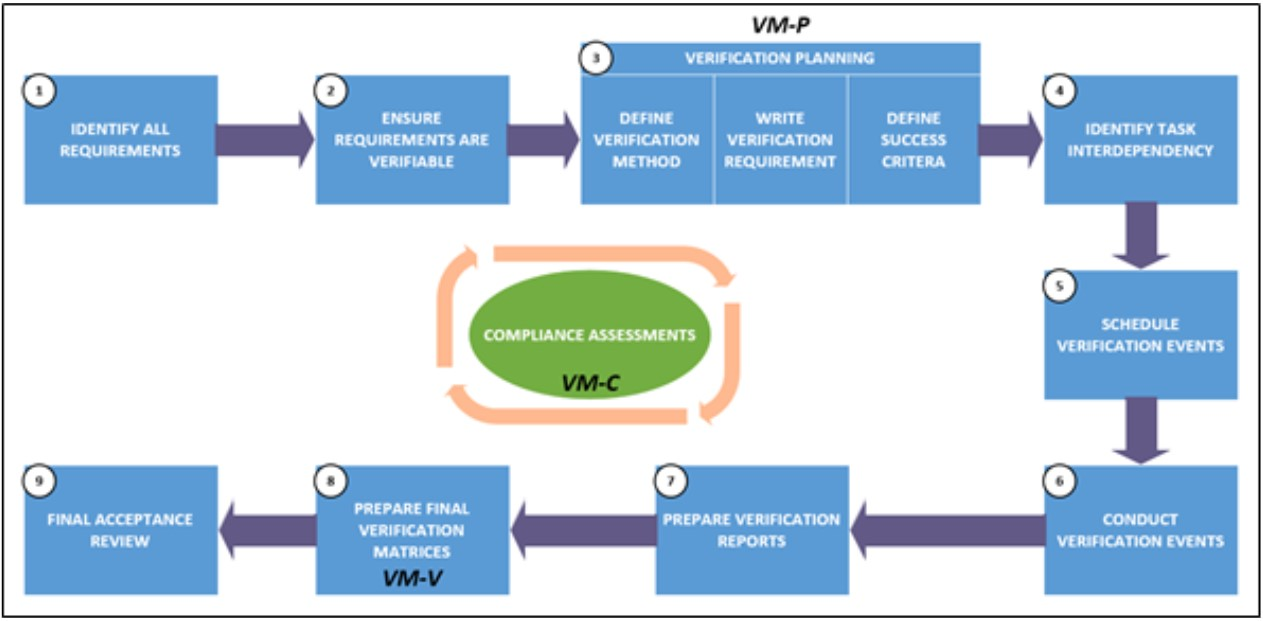
\includegraphics[width=0.5\textwidth]{static/verification_process}
    \caption{The Rubin Observatory Verification Process begins with Requirements Identification and ends with Final Acceptance Review}
    \label{fig:verification_process}
\end{figure}


\subsubsection{Rubin Operations Liaison to SIT-Com}
\label{sec:SCLT_liason_to_ops}

The Rubin Operations Liaison to SIT-Com exists to facilitate a smooth transition between Commissioning and Operations.
One of the primary roles is to assist in moderating the feedback between the on-going verification and characterization activities and the planning for the early stages of operations.
For example, this may include identifying the requirements which are most vital to the Operation's Team System Performance goals, then helping to priorize the appropriate system and/or science verification activities.
The Liaison will also assist in identifying missing or under-scoped activities (training, tools etc) from either of the construction and operations projects; then work together with both parties to derive appropriate coverage and/or mitigation.
It is expected that this person will also be the lead in acquiring operations related information for SIT-Com Teams and or working groups who would benefit from additional context and/or use-cases.

\section{SIT-Com Team Interactions}
\label{sec:interactions}
With the transition of the Rubin Project from the construction phase into commissioning, both the number of simultaneous activities and the global distribution of the participants has increased.
Understanding and managing the impacts of these activities on current and future schedules requires clear and regular communication both within the SIT-Com team and beyond.
As it is clearly impossible for all people to be in all meetings, a series of targeted meetings with key personnel and communication-specific agendas have been created to facilitate efficient information flow.
For ease of explanation, this section describes the interactions from a top-down direction.
However, the information flow during the meetings is bi-directional with the subsystem task identification, creation, assignment and prioritization done at the lower levels, whereas the scheduling and resource management discussions to balance global priorities occurs at a higher level.

\textbf{Strategic Planning Meeting}

\begin{itemize}
    \item Weekly cadence with $\sim$10 attendees
    \item Organized and executed by the Rubin Project Manager
    \item Attended by senior management of each subsystem, including at least two (but often all) of the SIT-Com Leads
    \item Identifies mid-to-long term priorities
    \item Communicates near-term issues (e.g. site restrictions or scheduled power outages) that may affect subsystem task selection and/or execution
    \item Assigns or shuffles resources (when required) to ensure task completion and that schedule is maintained
    \item Highest level meeting for conflict resolution discussions between subsystems with the ultimate decision authority resting with the Project Manager
\end{itemize}

\textbf{SIT-Com Leadership Team Meeting}

\begin{itemize}
    \item Weekly cadence with $\sim$10 SCLT members
    \item Additional attendees are occasionally invited for detailed technical discussions
    \item Organized and executed by SIT-Com Lead(s)
    \item Lead(s) present feedback from Strategic Planning Meeting on global priorities and recent events/impacts
    \item SIT-Com coordinators preset status, priorities, scheduling challenges, and require prerequisites, particularly those delivered by other subsystems
    \item Report of In-kind progress/findings
    \item SCLT jointly reviews priorities between groups and discusses task resourcing, prioritization and scheduling
\end{itemize}


\textbf{SIT-Com General Assembly Meeting}

\begin{itemize}
    \item Monthly cadence with $\sim$30+ attendees
    \item Scheduled for the first Monday of the month and replaces Leadership team meeting
    \item Executed by SIT-Com Lead(s) with content contributed by system coordinators
    \item Presents high-level project status, priorities and recent events that may impact SIT-Com activities
    \item System coordinators contribute slides on accomplishments, status and priorities
    \item Opportunity given to make calls for contributions or participation to events or activities
    \item When time permits, a presentation on a specific topic of broad interest may be given
\end{itemize}

\textbf{SIT-Com Product Owner Meeting}
\begin{itemize}
    \item Bi-Weekly cadence with $\sim$12 attendees
    \item Organized and executed by SIT-Com Software Integration System coordinators
    \item Expectation that this meeting replaces the T\&S PO meetings, therefore, most attendees will not have an additional meeting
\end{itemize}


\textbf{Commissioning Activity Planning Coordination Meeting}
\begin{itemize}
    \item Weekly cadence with $\sim$20 attendees
    \item Executed by SIT-Com Software Integration Lead
    \item Meeting is attended by numerous system coordinators and SIT-Com Product Owners
    \item Used to perform low-level prioritization of cross-subsystem software and IT related tasks
    \item Coordination of precise scheduling of  integration activities associated with the integration milestones
    \item Tracks progress of dependencies from multiple subsystems, most often (but not exclusively) related to software
\end{itemize}

\section{Task Management}
\label{sec:task_management}

The responsibility of task management primarily resides with a dedicated SIT-Com Lead who coordinates activities in close coordination with the system coordinators.
The identified Lead is responsible for both communicating and addressing issues brought up by the coordinators, but is in close contact with the other Leads and primarily acts as the primary representative and point-person.
Individual team members themselves are responsible for documenting their activities and providing a more accurate time estimate to completion.
The diverse nature of the tasks combined with the coordination of a large team necessitates the use of a task management tool.
Like the rest of the project, SIT-Com has adopted the use of Jira and is now working to derive an appropriate workflow that spans the multi-discipline and multi-faceted activities of the team.

Although the workflow is not yet finalized, the structure to facilitate it's operation is well-developed.
The global task priorities are defined first by a series of milestones, which are broken down into a series of tasks (epics), and ultimately into individual tasks.
The finer-grained week-to-week prioritization and coordination of the epics and subsidiary tasks are organized with input from the series of meetings (discussed in the previous section) with appropriate timeline estimates.
Each system coordinator, in collaboration with the SIT-Com team members carrying out the tasks, is then responsible for deriving, maintaining, and statusing the activities under their purview.
A roll-up of the status is reported each week at the SCLT meetings and timelines and/or the number of personnel working on a specific task are adjusted appropriately.
All work will be tracked in Jira and ultimately linked to SIT-Com milestones carried at the project level (in P6).

As mentioned previously, the detailing of the task management plan is currently under active development and this section will be updated in the next release of this document.

%Because SIT-Com is a collaboration of numerous individuals coming from different institutions, nearly all of whom work on other projects beyond Rubin Commissioning activities and have varying amounts of time devoted to Rubin Activities, it is
%Therefore, SIT-Com will not strictly follow the sprint planning and story-point accounting scheme that is typically used in Agile (software) development frameworks.
%Instead, the SCLT will define goals and present their priorities for each month during the General Assembly meeting.
%The system coordinators and team members will then align their tasks in accordance with those priorities and constraints and work with SIT-Com personnel to
%define sprints, with the number of activities being adapted to each team member.
%
%
%\textbf{Jira}
%\begin{itemize}
%    \item Need a work tracking tool with a managed backlog
%    \item M. Reuter can do the Jira setup work, but not the backlog management/prioritization
%    \item Needs more global input and to be assigned/tracked at numerous meetings
%    \item All COMs team members should have “sprints” - more to keep us on track than to evaluate efficiency etc.
%    \item Monthly (bi-monthly?) sprint planning meeting (which is big) should occur
%    \item Could add it on to the monthly meeting.
%    \item How do story-points work?
%    \item Do we need to implement this?
%    \item We need to at least estimate the type of resources needed and the time required.
%\end{itemize}


\subsection{Time Accounting}
\label{sec:time}

The time accounting and activity separation between subsystems and Commissioning (now SIT-Com) was previously defined in \citeds{LSE-70} as, ``An activity is considered part of commissioning when it involves a delivered component from one subsystem ``touching" that of another subsystem."
This also meant that if the SIT-Com team identified an issue or problem caused by a component delivered by a subsystem (e.g. the dome), it was responsibility of the subsystem (T\&S) to remedy the issue.
This definition proved useful for many years but is now no longer sufficiently detailed to address all questions and scenarios related to time accounting.
This section expands that definition and provides examples of how personnel and management make decisions regarding the charging of accounts for tasks performed by SIT-Com personnel.

There are several cases where the activity is clearly captured under the scope of SIT-Com, including:
\begin{itemize}
    \item Characterization of system performance, such as the effects of windshake, temperature, optimization of mirror position look-up tables, etc.
    \item Training to use subsystem tooling (e.g. scripting) should be charged to commissioning.
    This includes the subsystem person performing the training.
    \item The development of scripts or performing of tests that is used to characterize components and/or crosses subsystem boundaries (e.g. a standard visit script)
    \item Verification of functional aspects of any interface between subsystems (e.g. Camera to OCS)
\end{itemize}

Cases where the time should be charged to a subsystem WBS include:
\begin{itemize}
    \item Tasks involving delivery and verification of subsystem requirements
    \item Maintenance and/or repairs to subsystem deliverables
\end{itemize}

Where the division in time accounting becomes less obvious is during troubleshooting and verification/validation activities.
For example, performing characterization tests to track down and identify an issue with a component will charge SIT-Com.
The discussion and identification of the fix should also charge SIT-Com, however, the repair itself charges the subsystem.
A similar solution is to be utilized for the validation of cross-subsystem interfaces, functionality, and verification.
Under normal circumstances, this work is to be charged to SIT-Com, however, if validation fails, the discussion, identification and specification of what needs to get built gets charged to SIT-Com but an LCR should be filed to a subsystem to implement the changes or fix.

Lastly, the verification of functional aspects of an interface between components within a subsystem (E.g. M1M3 to TMA) is shared between the subsystem and commissioning.
These cases, which are limited in number, are to be worked out on a case-by-base basis between the SIT-Com and subsystem leads.

\subsection{Authorization and Activity Prioritization Management}

As discussed in previous sections, SIT-Com personnel are often working on multiple projects simultaneously, several of which may be for other subsystems and guided by different lines of reporting.
This section describes how the various demands on personnel are identified, raised, discussed, decided, and communicated.

As discussed in section \ref{sec:interactions}, there are numerous meetings where global project priorities are discussed, these conversations include demands on personnel and efforts are made to identify and negotiate the division of time before detailed planning at the individual task level.
In most cases, this avoids the employee from having to individually navigate the prioritization of their tasks.
In cases where management does not identify the conflict early on, it is up to the employee to voice their concerns regarding priority, availability, workload, timeline etc. to both supervisors.
Ideally this will happen simultaneously via email or via a direct discussion.
Once raised, a discussion between the employee's administrative supervisor and one of the SIT-Com Leads ensues; the employee is not responsible for making the decision regarding which task takes priority.
Although other factors may be at play, the decision should be largely based upon the project's global priorities which are outlined as part of the Wednesday meeting described in section \ref{sec:interactions}.
In the case where the supervisors are unable to reach a unanimous decision, the issue gets elevated to the Program Manager.

\subsection{Summit Work Authorization}
Performing summit related tasks require an additional step for authorization as summit activity authorization and prioritization is managed via the SUMMIT Jira process.
The global priorities flow down from the Wednesday Strategic Planning Meeting and are then balanced against available resources in the Thursday Summit Planning meeting; a meeting attended by numerous SIT-Com personnel.
Activities that are to take place on the summit must be approved via this process to minimize and mitigate impacts to summit activities and to ensure safety of personnel.

The interactions and workflows of the SIT-Com and SUMMIT Jira projects is now being developed.

\subsection{Verification Management}

The Verification and Validation process is primarily managed within our Verification Architecture which is presented graphically in Figure \ref{fig:verification_arch}.
The Verification Architecture is composed of 3 primary components: MagicDraw model, Jira with Test Manager, and Syndeia.
The high level verification planning is performed in the MagicDraw model.
The requirements are decomposed into 1 or more Verification Elements.
The Verification Elements are traced to Verification Procedures.
The Verification Procedures are organized and sequenced into Verification Cycles.
The Verification Cycles are organized into Verification Plans.
These elements are then synced into Jira using Syndeia.
The detailed planning of the exact steps to be executed within a verification procedure is done within the Jira Test Manager system.
The Verification Plans align with a Verification Event which is executed in Jira via the execution of the Verification Cycles.
The results of the Verification Events are captured in a SIT-COM Test Plan / Test Report (SCTR) are generated from the information in Jira and pushed to \href{https://lsst.io}{lsst.io} and then archived in DocuShare.
The results from Jira are then synced back into MagicDraw using Syndeia.

\begin{figure}[h]
    \centering
    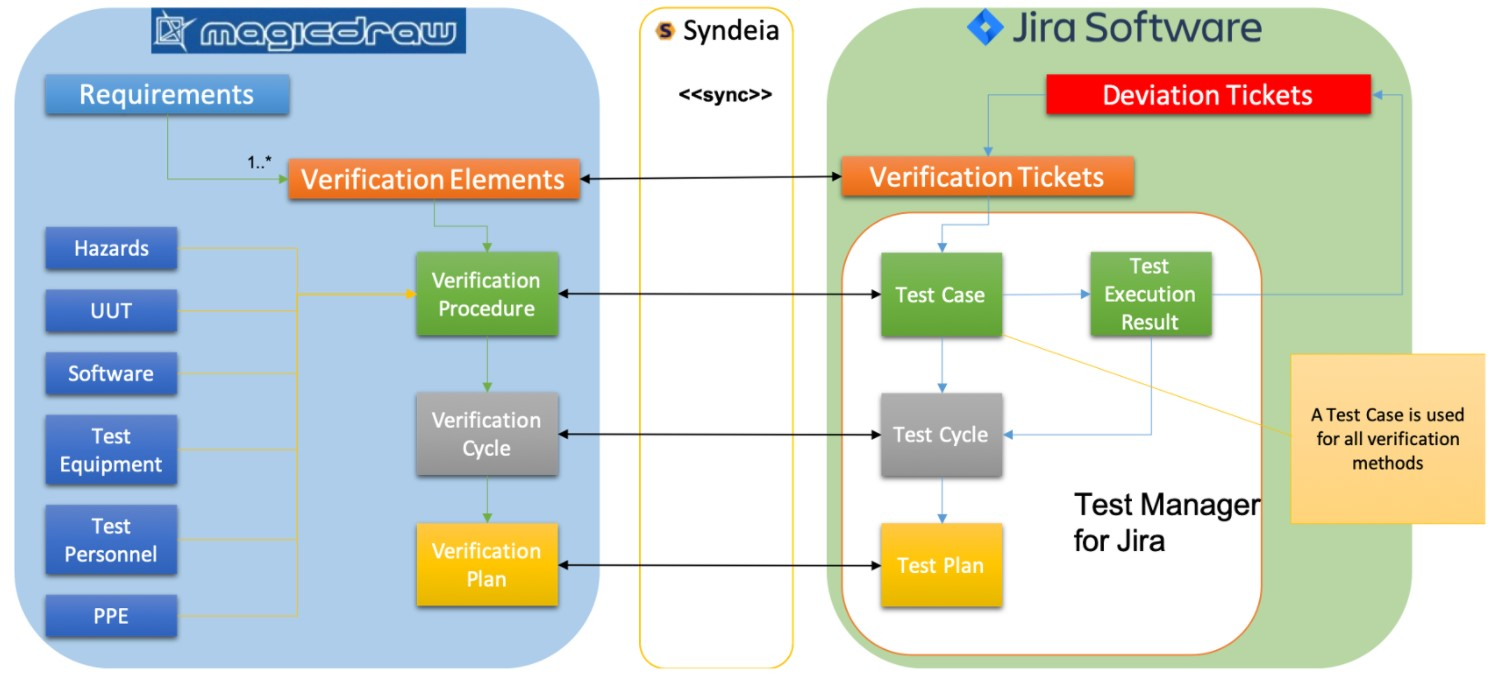
\includegraphics[width=0.5\textwidth]{static/verification_architecture}
    \label{fig:verification_arch}
    \caption{The Verification Architecture Overview.}
\end{figure}

The workflow for the verification tickets in Jira enforces the verification process through transition conditions, transition validations, and the evaluations of tickets and test cases linked to the verification ticket.
This is shown in Figure \ref{fig:verification_workflow}.

\begin{figure}[h]
    \centering
    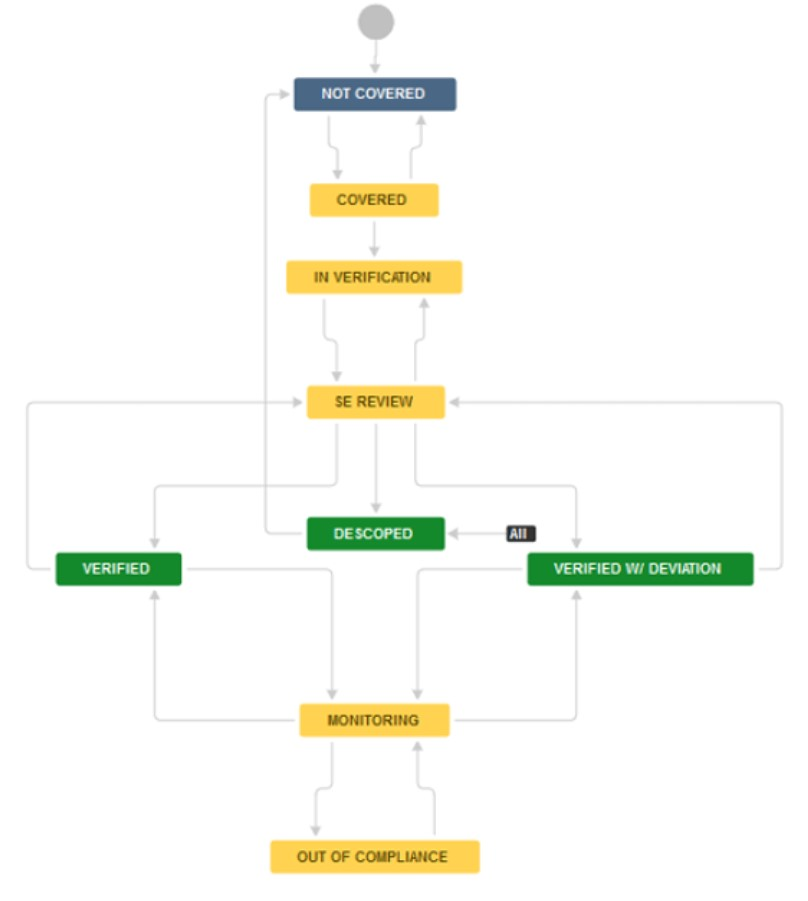
\includegraphics[width=0.5\textwidth]{static/verification_workflow}
    \caption{The Jira Verification Ticket Workflow.}
    \label{fig:verification_workflow}
\end{figure}

The full details of the Rubin Observatory Verification Process is described in \citeds{LSE-160}.

%\subsection{Software Code Management}
%
%\textbf{This should go probably go in a technote.}
%\begin{itemize}
%    \item Outline that we follow DM and T\&S development practices
%    \item Expectations of commissioning personnel and their interaction with the software system for characterization testing is in tstn-024
%    \item Contribution of how commissioning team code gets incorporated is in tstn-010
%    \item Configuration changes by commissioning personnel (and others) follow tstn-017
%    \item Repo management?  Identify resources that are need but not present in the Project
%\end{itemize}

\section{Environment, Health and Safety}

The Rubin Safety Policy (\citeds{LPM-18}) will continue to be the guiding document that defines Rubin's safety culture, expected safety behaviors, and details the broad responsibilities for all those who work for Rubin.
The Rubin Project is centrally managed but executed by several teams in distributed locations and with different funding sponsors.
This Rubin Safety Policy covers all Rubin Project efforts while recognizing and relying on existing Safety,
Health and Environmental policies in place at participating institutions.

Given that environmental conditions on the summit can be uncomfortable and activities can be complex, the Summit Site Safety, Health, and Environmental Plan (\citeds{LPM-114}) details required communications, minimum safety processes and procedures.
Due to the varied activities that will be occurring on the summit, the following processes will be enforced: 1) Work Stop Authority, 2) the morning Plan of the Day, and 3) the overarching authority to direct work of the Site Manager.  In addition, many other safety control processes will be in place, including but not limited to:
\begin{itemize}
    \item Known hazards are recognized in the Rubin Hazard Analysis process and are mitigated or minimized;
    \item All employees working in Chile will have an ODI (obligation to inform) to understand the hazards of their job;
    \item All employees working in Chile are required to attend general safety training specific to working at the site and trained for specific hazards related to their work such as lock out-tag out;
    \item All procedures will include hazard recognition, safety equipment needed and mitigation strategies.
\end{itemize}


\section{Risks and Hazards in Commissioning}
\subsection{Risks}
SIT-Com will maintain a shared risk registry developed using the template of the DOE MIE project risk registry (\citeds{LCA-30}).
The risk analysis follows key concepts presented in both the Camera Risk Management Plan (LCA-29) and the Rubin Risk and Opportunity Management Plan (\citeds{LPM-20}).
Risks and contingent events can affect the commissioning schedule and budget; managing risks is essential and helps determine sufficiency of contingency funding.

The bottom up estimates for scheduled work are, as required, success oriented.
SIT-Com has intentionally budgeted in small periods of time to resolve expected minor issues.
We cannot foresee which risks will be realized.
Rather, the risk registry allows us to evaluate the impacts of each risk if realized and to fund risk reduction activities.

\subsection{Hazards}
The safety of people and property is paramount in all Rubin efforts.
The design for safety has included assembly and construction processes and the resulting commissioning and operational concepts.
As procedures are developed for the observatory, job hazard analysis will be included to protect people, equipment, and processes from known hazards.


\appendix

% Include all the relevant bib files.
% https://lsst-texmf.lsst.io/lsstdoc.html#bibliographies
\section{References} \label{sec:bib}
\renewcommand{\refname}{} % Suppress default Bibliography section
\bibliography{local,lsst,lsst-dm,refs_ads,refs,books}

% Make sure lsst-texmf/bin/generateAcronyms.py is in your path
\section{Acronyms} \label{sec:acronyms}
\addtocounter{table}{-1}
\begin{longtable}{p{0.145\textwidth}p{0.8\textwidth}}\hline
\textbf{Acronym} & \textbf{Description}  \\\hline

AIV & Assembly Integration and Verification \\\hline
ComCam & The commissioning camera is a single-raft, 9-CCD camera that will be installed in LSST during commissioning, before the final camera is ready. \\\hline
DM & Data Management \\\hline
DOE & Department of Energy \\\hline
EFD & Engineering and Facility Database \\\hline
EVMS & Earned Value Management System \\\hline
FRACAS & Failure Reporting Analysis and Corrective Action System \\\hline
HSC & Hyper Suprime-Cam \\\hline
IN2P3 & Institut National de Physique Nucléaire et de Physique des Particules \\\hline
IT & Information Technology \\\hline
LCA & Document handle LSST camera subsystem controlled documents \\\hline
LCR & LSST Change Request \\\hline
LPM & LSST Project Management (Document Handle) \\\hline
LSE & LSST Systems Engineering (Document Handle) \\\hline
LSR & LSST System Requirements; LSE-29 \\\hline
LSST & Legacy Survey of Space and Time (formerly Large Synoptic Survey Telescope) \\\hline
LVV & LSST Verification and Validation \\\hline
M1M3 & Primary Mirror Tertiary Mirror \\\hline
MIE & Major Item of Equipment \\\hline
MREFC & Major Research Equipment and Facility Construction \\\hline
NSF & National Science Foundation \\\hline
OCS & Observatory Control System \\\hline
OSS & Observatory System Specifications; LSE-30 \\\hline
PEP & Project Execution Plan \\\hline
PO & Program Operations \\\hline
PSE & Project Systems Engineering \\\hline
QA & Quality Assurance \\\hline
SE & System Engineering \\\hline
SIT & System Integration, Test \\\hline
SIT-COM & System Integration, Test and Commissioning \\\hline
SV & Science Validation \\\hline
T\&S & Telescope and Site \\\hline
TBD & To Be Defined (Determined) \\\hline
TBR & To Be Resolved \\\hline
TCS & Telescope Control System \\\hline
TMA & Telescope Mount Assembly \\\hline
US & United States \\\hline
WBS & Work Breakdown Structure \\\hline
\end{longtable}

% If you want glossary uncomment below and comment out the two lines above.
% \printglossaries

\end{document}
